\section{Introduction}
% (this \section triggers the automatic divider frame defined above)

% ---------- Slide: The Hook ----------
\begin{frame}{A Familiar Problem}

\begin{columns}[T,onlytextwidth]

\begin{column}{0.44\textwidth}
\centering
\begin{tikzpicture}[
  every node/.style={circle, draw=oc-gray-6, thick, minimum size=0.9cm, font=\bfseries\small},
]
  \node (A) at (0,2.1)    {A};
  \node (B) at (1.6,2.1)  {B};
  \node (C) at (0,0.6)    {C};
  \node (D) at (1.6,0.6)  {D};
  \node (E) at (0,-0.9) {E};

  \draw<2->[oc-blue-6, thick] (A) -- (B);
  \draw<3->[oc-blue-6, thick] (C) -- (D);
  \draw<3->[oc-blue-6, thick] (C) -- (E);

  \draw<5->[oc-red-9, densely dashed, thick] (A) -- (D);

  \draw<4->[oc-teal-6, line width=2pt, rounded corners] (D) -- (C) -- (E);
  \node<4->[draw=oc-teal-6, thick] at (D) {D};
  \node<4->[draw=oc-teal-6, thick] at (E) {E};

  \node<5->[draw=oc-red-9, thick] at (A) {A};
  \node<5->[fill=structure.bg, circle, inner sep=1.5pt] at ($(A)!0.5!(D)$)
    {\textcolor{oc-red-9}{\footnotesize\faIcon{times}}};
\end{tikzpicture}
\end{column}

\begin{column}{0.54\textwidth}
\begin{itemize}
  \item<1-> Suppose there are five students in a classroom.
  \item<1-> At first, none of them know one another.
  \item<2-> A and B become friends.
  \item<3-> Separately, C become friends with D and E.
  \item<4-> \alert{Are D and E friends?} Yes --- indirectly, through C, they belong to same friend circle.
  \item<5-> What about \alert{A and D}? No --- they belong to two different circles entirely.
\end{itemize}
\end{column}

\end{columns}

\end{frame}

% ---------- Slide: Naming the Solution ----------
\begin{frame}{Larger Networks}
 
\begin{columns}[T,onlytextwidth]
 
\begin{column}{0.46\textwidth}
\begin{figure}[h]
    \centering
    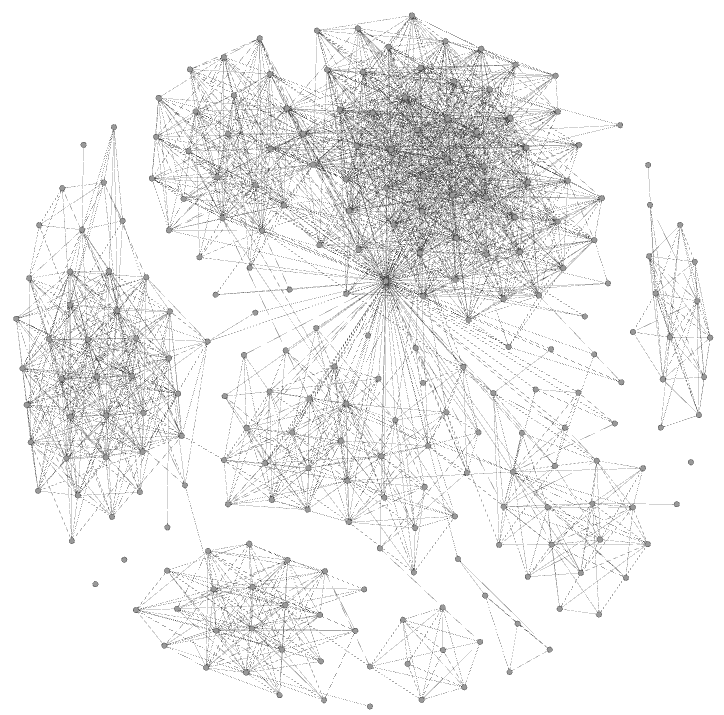
\includegraphics[width=0.95\linewidth]{social_network.png}
    {\tiny\itshape\color{oc-gray-6} \caption{Social Media Network Visualization\footnote{Pinterest: Visualise Your Facebook Friend Network}}}
    \label{fig: social_network}
\end{figure}

\end{column}
 
\begin{column}{0.50\textwidth}
\begin{itemize}
  \item<1-> Consider a large social network, or equally, a large computer network, with countless members.
  \item<2-> We need to answer \textbf{efficiently}: \alert{are any two given members connected?}
\end{itemize}
 
\vspace{6pt}
\onslide<3->{%
\begin{tcolorbox}[colback=oc-blue-0, colframe=oc-blue-6, boxrule=0.8pt, arc=1.5pt, left=6pt, right=6pt, top=4pt, bottom=4pt]
\centering\large\textbf{This is exactly what \emph{Disjoint Set Union} answers.}
\end{tcolorbox}%
}
\end{column}
 
\end{columns}
 
\end{frame}

\begin{frame}{What Is a Disjoint Set Union?}

\begin{columns}[T,onlytextwidth]

\begin{column}{0.52\textwidth}
\centering
\begin{tikzpicture}[
  member/.style={circle, draw=oc-gray-6, fill=white, thick, minimum size=0.65cm, font=\bfseries\small},
  leader/.style={member, double, double distance=1pt, line width=1pt, text=white},
  set label/.style={font=\small\bfseries}
]
  \path[use as bounding box] (-0.2,-0.5) rectangle (5.8,4.3);

  \draw<1->[draw=oc-blue-6, fill=oc-blue-0, thick]
    (0,2.4) .. controls (-0.2,3.0) and (0.1,4.0) .. (0.8,4.0)
    .. controls (1.5,4.2) and (2.5,4.0) .. (2.5,3.3)
    .. controls (2.7,2.5) and (2.0,2.1) .. (1.3,2.2)
    .. controls (0.7,2.0) and (0.2,2.0) .. cycle;
  \node<1->[member] at (0.65,3.35) {A};
  \node<1->[member] at (1.8,3.4) {B};
  \node<1->[member] at (1.25,2.6) {C};
  \node<1->[set label, text=oc-blue-6] at (1.25,4.2) {$S_1$};

  \draw<1->[draw=oc-teal-6, fill=oc-teal-0, thick]
    (3.1,2.7) .. controls (2.8,3.4) and (3.3,4.1) .. (4.0,4.0)
    .. controls (4.7,4.2) and (5.6,3.8) .. (5.5,3.2)
    .. controls (5.7,2.4) and (5.0,2.1) .. (4.3,2.2)
    .. controls (3.6,2.0) and (3.2,2.2) .. cycle;
  \node<1->[member] at (3.65,3.35) {D};
  \node<1->[member] at (4.8,3.4) {E};
  \node<1->[member] at (4.25,2.6) {F};
  \node<1->[set label, text=oc-teal-6] at (4.25,4.2) {$S_2$};

  \node<2->[leader, draw=oc-blue-6, fill=oc-blue-6] at (0.65,3.35) {A};
  \node<3->[leader, draw=oc-teal-6, fill=oc-teal-6] at (3.65,3.35) {D};

  \node<2->[
    font=\footnotesize,
    text=oc-gray-6,
    text width=6cm,
    align=left
] at (3.2,-0.4)
{
    Here,
    \begin{itemize}
        \item<2-> $A$ is the representative of $S_1$
        \item<3-> $D$ is the representative of $S_2$
    \end{itemize}
};
\end{tikzpicture}
\end{column}

\begin{column}{0.44\textwidth}
\textbf{Definition}
\begin{itemize}
  \item Sets are \alert{disjoint} if they share no elements:
    \[S_i \cap S_j = \varnothing \quad \text{for } i \ne j.\]
  \item \textbf{Disjoint Set Union} or \textbf{DSU} are a collection of such disjoint groups.
\end{itemize}

\vspace{6pt}
\onslide<2->{%
\textbf{Representative (``leader'')}
\begin{itemize}
  \item One chosen element identifies the entire set.
\end{itemize}
}
\onslide<4->{%
\begin{tcolorbox}[colback=oc-blue-0, colframe=oc-blue-6, boxrule=0.8pt, arc=1.5pt, left=6pt, right=6pt, top=4pt, bottom=4pt]
\centering\small
Same representative $\Longleftrightarrow$ same set.
\end{tcolorbox}%
}
\end{column}

\end{columns}

\end{frame}

% ---------- Slide 5: The Interface ----------
\begin{frame}{The Interface}

  \begin{enumerate}
    \item<1-> \texttt{make\_set(x)}
      \begin{itemize}
        \item<1-> Creates a new set whose only member is \texttt{x}.
      \end{itemize}

    \vspace{10pt}
    \item<2-> \texttt{find(x)}
      \begin{itemize}
        \item<2-> Returns the representative of the set containing \texttt{x}.
      \end{itemize}

    \vspace{10pt}
    \item<3-> \texttt{union(x, y)}
      \begin{itemize}
        \item<3-> Merges the sets containing \texttt{x} and \texttt{y} into one.
      \end{itemize}
  \end{enumerate}

  \vspace{14pt}
  \onslide<4->{%
    \begin{tcolorbox}[colback=oc-blue-0, colframe=oc-blue-6, boxrule=0.8pt, arc=1.5pt, left=6pt, right=6pt, top=4pt, bottom=4pt]
        Bacause of the two main operations, \texttt{union} and \texttt{find}, this structure is also called \textbf{Union--Find}.
    \end{tcolorbox}
  }

\end{frame}